\documentclass[pdftex,11pt,a4paper]{article}
\usepackage[pdftex]{graphicx}
\usepackage{fancyhdr}
\usepackage{geometry}
\usepackage{draftcopy}
\usepackage{float}
\usepackage{amsmath}
\usepackage{algorithm2e}

\renewcommand{\thesection}{\arabic{section}.}
\renewcommand{\thesubsection}{\arabic{section}.\arabic{subsection} }
\renewcommand{\headrulewidth}{0pt}
\renewcommand{\footrulewidth}{0.5pt}
\pagestyle{fancy}
\fancyhead{}
\fancyfoot[LE,LO]{\footnotesize{
SE344, Chemistry and Our Environment
}
}

\title{\vspace{-15pt}Greenhouse Gases and Energy Balance of Earth\\ SE344: Chemistry and Our Environment}
\author{Ankesh Kumar Singh (Y9090)}
\date{31st January, 2013}
\begin{document}
\maketitle
\begin{tabular}{p{370pt}}
\textbf{Keywords: }Greenhouse effect, Greenhouse gases, Albedo, climate change, global warming, earth's energy budget
\end{tabular}
\vspace{10pt}\\
\hrule
\vspace{10pt}
The main source of energy to earth is the sun. At the top of atmosphere, radiations are received as shortwaves, some of it is reflected by clouds and most of it is transmitted. Upper atmosphere does not absorb these radiations and therefore they heat earth’s surface. The reflected longwaves from the surface maintain a delicate balance of energy on earth.\\

\textbf{Albedo}, or reflection coefficient is defined as the ratio of reflected radiation from the surface to incident radiation upon it. Being a dimensionless fraction, it may also be expressed as a percentage, and is measured on a scale from zero for no reflecting power of a perfectly black surface, to 1 for perfect reflection of a white surface.\\

\textbf{Greenhouse effect} is a process by which thermal radiations emitted by the earth’s surface are absorbed by the atmosphere and re-radiated in all directions. Since a part of these gases are radiated back to the surface, it leads to elevation in the temperature of troposphere, the layer of atmosphere closest to the surface. The gases which cause this effect are called greenhouse gases. Greenhouse effect is essential for life forms to survive on earth. Typically, earth’s temperature is 33$^o$C more than what it would have been without greenhouse effect.\\

Water vapor has highest absorptivity among all greenhouse gases, but we do not consider it as a pollutant. This is because it is essential for the sustaining life and it is also regulated by precipitation. Carbon dioxide on the other hand has a significant contribution, followed by methane. CO$_2$ is produced from fossil fuel burning and increasing deforestation. Plants are able to fix CO$_2$ into glucose using sunlight as form of energy, in the process of photosynthesis, releasing O$_2$.
$$6\,CO_2+6\,H_2O\rightarrow  C_6H_{12}O_6+6\,O_2$$
\begin{figure}[htb]
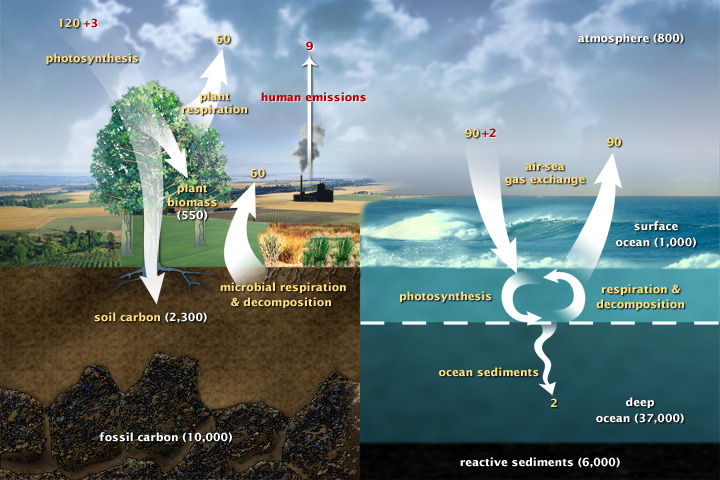
\includegraphics[clip=true,trim=0pt 0pt 0pt 0pt,scale=0.58]{Carbon_cycle.jpg}
\caption{Carbon cycle}
\center{\textit{Source: }http://earthobservatory.nasa.gov/Features/CarbonCycle/}
\end{figure}
Oceans serve as another important sink for CO$_2$, by converting it into carbonates and bicarbonates.
Anthropogenic increase has contributed to 30\% rise in CO$_2$ content of the atmosphere. The global carbon cycle is now usually divided into the following major reservoirs of carbon interconnected by pathways of exchange:
\begin{itemize}
\item atmosphere
\item terrestrial biosphere
\item oceans, including dissolved inorganic carbon and living and non-living marine biota
\item sediments, including fossil fuels, fresh water systems and non-living organic material, such as soil carbon
\item Earth's interior, carbon from the Earth's mantle and crust
\end{itemize} 

These carbon stores interact with the other 
components through geological processes
The carbon exchanges between reservoirs occur as the result of various chemical, physical, geological, 
and biological processes. The ocean contains the largest active pool of carbon near the surface of the Earth. 
The natural flows of carbon between the atmosphere, ocean, and sediments is fairly balanced, so that carbon levels 
would be roughly stable without human influence.\\

Methane as greenhouse gas is produced from rice cultivation, cattle and sheep ranching, decay from landfills and mining. Anthropogenic increase contributes to 145\% methane. Average atmos. residence time for methane is 7-10 years. N$_2$O is emitted from industries and fertilizers used in agriculture. Average atmos. residence time for N$_2$O is 140-190 years.\\

Temperatures have risen by 1$^o$C over last 100 years. This has led to an ecological imbalance. There is no way of predicting how this would affect the ecosystem and whether the change is likely to speed up in the near future. Climatic conditions affect production, which directly affects prices. Thus, global climate change is an important parameter to be incorporated in a good financial model.
\end{document}